\chapter{Software}
\label{ch:software}


% %
% HEADER
% %
\lipsum[1]


% %
% INSTALLATION
% %
\section{Installation}
\label{sec:installation}

\lipsum[1]


% %
% CONFIGURATION
% %
\section{Configuration}
\label{sec:configuration}

\lipsum[1]


% %
% DEPLOYMENT
% %
\section{Deployment}
\label{sec:deployment}

\lipsum[1]


% %
% USAGE
% %
\section{Usage}
\label{sec:usage}

\lipsum[1]


% %
% FIGURE
% %
\section*{Figure}

\begin{figure}	
	\label{fig:sample-figure}
	\centering
	
\includegraphics[width=.7\columnwidth]{sample-figure}
	\caption{Lorem ipsum dolor sit amet, consectetur adipiscing elit, sed do eiusmod tempor incididunt ut labore et dolore magna aliqua. Ut enim ad minim veniam, quis nostrud exercitation ullamco laboris nisi ut aliquip ex ea commodo consequat.}
\end{figure}

% %
% PLOT
% %
\section*{Plot}

\begin{figure}	
	\label{fig:sample-bar}
	\centering
	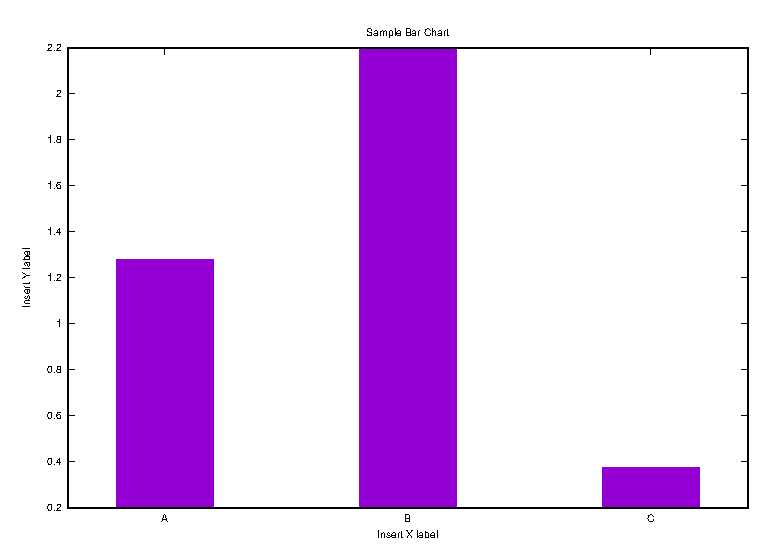
\includegraphics[width=.7\columnwidth]{bar}
	\caption{Lorem ipsum dolor sit amet, consectetur adipiscing elit, sed do eiusmod tempor incididunt ut labore et dolore magna aliqua. Ut enim ad minim veniam, quis nostrud exercitation ullamco laboris nisi ut aliquip ex ea commodo consequat.}
\end{figure}

\begin{figure}	
	\label{fig:sample-line}
	\centering
	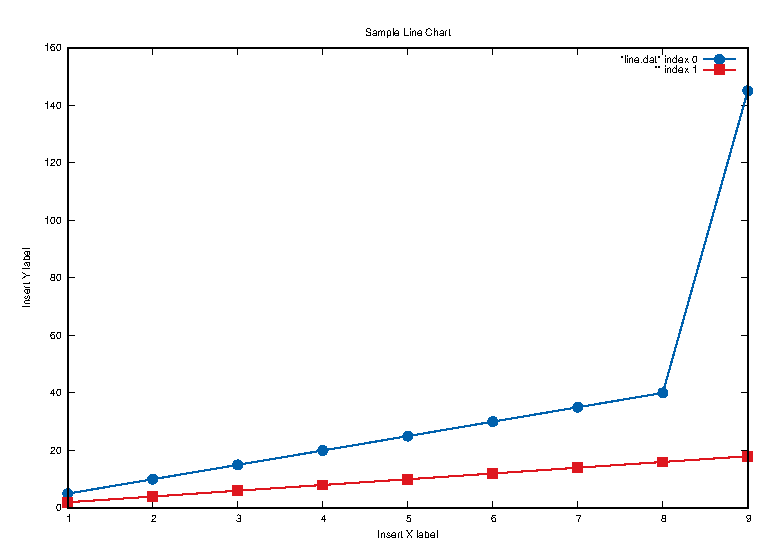
\includegraphics[width=.7\columnwidth]{line}
	\caption{Lorem ipsum dolor sit amet, consectetur adipiscing elit, sed do eiusmod tempor incididunt ut labore et dolore magna aliqua. Ut enim ad minim veniam, quis nostrud exercitation ullamco laboris nisi ut aliquip ex ea commodo consequat.}
\end{figure}

% %
% EQUATION
% %
\section*{Equation}


\begin{eqnarray*}
	a_i & = & a_j + a_k \\
	a_i & = & 2a_j + a_k \\
	a_i & = & 4a_j + a_k \\
	a_i & = & 8a_j + a_k \\
	a_i & = & a_j - a_k \\
	a_i & = & a_j \ll m \mbox{shift}
\end{eqnarray*}


% %
% TABLE
% %
\section*{Table}

\begin{table}
	\caption{Armadillos}
	\label{arm:table}
	\begin{center}
		\begin{tabular}{||l|l||}\hline
			Armadillos & are \\\hline
			our	   & friends \\\hline
		\end{tabular}
	\end{center}
\end{table}

% %
% ALGORITHM
% %
\section*{Algorithm}

\begin{algorithm}[t]
	\label{alg:parser}
	\SetKwProg{Fn}{Function}{}{}  
	
	\Fn{parse (grammar,ontology,question)} {
		$state \leftarrow new\; ParserState(question)$ \\
		$tokenizer \leftarrow new\; Tokenizer(grammar,question)$ \\
		
		\While{$token = tokenizer.next()$}{
			$candidates \leftarrow token.candidates$ \\
						\If{$candidates.size = 1$}{
				$candidate \leftarrow candidates.get(0)$ \\
				\ElseIf{$isSentence(candidate)$}{
					\If{$\neg state.curr = NULL$}{
						Error(multiple sentence root found) \\
					}
					$state.curr \leftarrow candidate$ \\
				}
				\Else{
					produce(state,candidate)
				}
			}
			
			\For{$ambiguity \in state.ambiguities$}{
				solveAmbiguity(state,ontology,ambiguity) \\
			}
		}
		\KwResult{$curr$}
	}
	\caption{Pseudocode of the \texttt{AlgorithmName}.}
\end{algorithm}

\clearpage
\newpage